The previous section demonstrates the RF modules that involve  the communication between PCD and PICC. This section will describe in detail each module of the Analog Front End for ISO/IEC 14443A (see Fig. \ref{fig:afe}).

\begin{figure}[]
  \centering
  \includegraphics[page=10,width=80mm]{images-crop.pdf}
  \caption{PICC Analog Front End}
  \label{fig:afe}
\end{figure}

\subsection{Power Supply Generator (PSG)}

The Power Supply Generator splits into two parts: signal rectification and power limitation.

The first part rectifies the RF field signal to get power supply for the chip. And the second part consists a Shunt resistor. The Shunt resistor is capable to limit the voltage of the antenna and protects the whole chip. ISO/IEC14443-2 requires the PICC to work when magnetic intensity between 1.5-7.5A/m rms. Therefore the PICC must work in these extreme conditions.  

The simplified schematic of signal rectification is shown in Fig. \ref{fig:rect} and power limitation (Shunt resistor) is shown in Fig. \ref{fig:shunt}.

\begin{figure}[h]
  \centering
  \includegraphics[page=11,width=60mm]{images-crop.pdf}
  \caption{Full Wave Rectifier}
  \label{fig:rect}
\end{figure}

\begin{figure}[h]
  \centering
  \includegraphics[page=12,width=60mm]{images-crop.pdf}
  \caption{Shunt Resistor}
  \label{fig:shunt}
\end{figure}

\subsection{Clock Generator (CG)}

The Clock Generator recovers the clock from the antenna and is used by the DPU. This module generates a clock source of 13.56 MHz. Basically consists of two FF/D and a XOR logic gate. 

The difference of phase between RF+ and RF- are 180 degrees, it is easy to take advantage of this property to recompose the clock. The simplified schematic is shown in Fig. \ref{fig:clk} and the simulation in the Fig. \ref{fig:clk_sim}.

\begin{figure}[]
  \centering
  \includegraphics[page=13,width=60mm]{images-crop.pdf}
  \caption{Clock Generator schematic}
  \label{fig:clk}
\end{figure}

\begin{figure}[]
  \centering
  \includegraphics[page=14,width=80mm]{images-crop.pdf}
  \caption{Clock recovery simulation}
  \label{fig:clk_sim}
\end{figure}

\subsection{Voltage Regulator (VR)}

The Voltage Regulator is a Low Dropout (LDO) Regulator. The topology is shown in Fig. X. Basically it consist of a reference source, in this case, a beta multiplier is used for this purpose. The OP AMP play the role of controller, it copies the reference voltage, control the variation of VRECT or VDD and reflects the reference voltage to the output.

\begin{figure}[]
  \centering
  \includegraphics[page=15,width=60mm]{images-crop.pdf}
  \caption{Voltage Regulator schematic}
  \label{fig:ldo}
\end{figure}

\subsection{Modulator}

The modulator transmits the signal from PICC to PCD. There are two different types of load modulation: resistive and capacitive modulation. Both types create a subcarrier next to 13.56MHz. Resistive modulation was adopted in this design for its simplicity. The schematic is shown in Fig. \ref{fig:mod}.

\begin{figure}[h]
  \centering
  \includegraphics[page=16,width=40mm]{images-crop.pdf}
  \caption{Modulator schematic}
  \label{fig:mod}
\end{figure}

\subsection{Demodulator}

The demodulator recovers the digital signals from the ASK signal transmitted from PCD. An Envelope Extractor (EE) is needed to extract the data. The digital signal is recovered by connecting the output of the EE with the input of the buffer.  The circuit is shown in Fig. \ref{fig:demod}. 

\begin{figure}[h]
  \centering
  \includegraphics[page=17,width=80mm]{images-crop.pdf}
  \caption{Demdulator schematic}
  \label{fig:demod}
\end{figure}

\subsection{Power On Reset (POR)}

The Power On Reset module is used to reset the digital machine and put it into idle state. It consists of a RC low pass network. The schematic is demonstrated in Fig. \ref{fig:por}. 

\begin{figure}[h]
  \centering
  \includegraphics[page=18,width=20mm]{images-crop.pdf}
  \caption{POR schematic}
  \label{fig:por}
\end{figure}